\documentclass[11pt,a4paper]{report}
\usepackage[utf8]{inputenc}
\usepackage[T1]{fontenc}
\usepackage[english]{babel}
\usepackage{amsmath}
\usepackage{amsfonts}
\usepackage{amssymb}
\usepackage{color}
\usepackage{graphicx}
\usepackage{url}
%\usepackage{subfig}
\usepackage{subfigure}
\usepackage[pagestyles]{titlesec}
\usepackage{geometry}

\author{Supervisor: Pr. Yahya Tayalati \\ Student: Faissal BAHMANE}
\setcounter{secnumdepth}{1}

%\titleformat{\chapter}[display]{\normalfont}{}{0pt}{\Large}


\begin{document}

	\begin{titlepage}

		\newcommand{\HRule}{\rule{\linewidth}{0.5mm}}
		\center
		\textsc{\LARGE CERN summer student report 2022}\\[1.5cm]

		\HRule \\[0.4cm]
		{ \huge \bfseries Geant4 simulations with ML}\\[0.4cm]
		\HRule \\[1.5cm]

		\begin{minipage}{0.4\textwidth}
			\begin{flushleft} \large
				\emph{Author:}\\
				Faissal \textsc{BAHMANE} % Your name
			\end{flushleft}
		\end{minipage}
		~
		\begin{minipage}{0.4\textwidth}
			\begin{flushright} \large
				\emph{Supervisor:} \\
				Pr. Yahya \textsc{TAYALATI}
			\end{flushright}
		\end{minipage}\\[2cm]

		{\large \today}\\[2cm]

		
\includegraphics[scale=0.25]{imgs/um6p_logo.png}
		\hfill
		
\includegraphics[scale=0.4]{imgs/msda_logo.png}
		\vfill
		
\includegraphics[scale=0.6]{imgs/CERN_logo_white.png}
		\hfill
		\includegraphics[scale=0.5]{imgs/atlas_logo.png}

		\vfill

	\end{titlepage}

	\tableofcontents

	\chapter{\sc Introduction}
	This project is about implementing simulations of the interaction of particles inside detectors using the Geant4 toolkit, the goal is to use machine learning based models to generate simulations of the interaction and to study speed of the simulation. In the project we try to simulate multiple types of particles with different ranges of energy and measure the energy deposition inside the detector. The bulk of my project was dedicated to learn how the Geant4 toolkit work and how we can generate machine learning based simulations inside the Geant4 toolkit. In the first section we introduce the Geant4 toolkit and explain the basics of the API and how to implement a simulation inside Geant4. In the second section we explain an example simulation of a beam of particles interacting with a detector composed of water and records the energy deposition of particles in each voxel of the detector. The third section is about Parametrization capability of Geant4 that allows the inhibition of the tracking process thereby allowing the use of an external inference model to generate the tracks and the deposition of energy. In the last section we present some perspectives of the project, presenting some ideas of the use of machine learning techniques for particle simulation.

	\chapter{\sc Geant4 Toolkit}

	\begin{center}
		
\includegraphics[scale=1]{imgs/g4logo.png}
	\end{center}
	Geant4\footnote{\url{https://geant4.web.cern.ch/}} is a C++ based toolkit used for the simulation of interaction of particles through matter using Monte Carlo methods. It is used in High Energy Physics, accelerator physics and also in medical science. It is maintained by the Geant4 collaboration and its source code is freely available under the Geant4 License.

	The toolkit has wide range of functionalities like tracking, geometry, physics models and hits. It supports multiple physical processes including electromagnetic processes, optical processes and hadronic processes. It also supports multiple types of particles, materials and elements, covering a range of energy starting from $250$ eV and reaching the TeV range.

	Geant4 is implemented in C++ with Object-Oriented paradigm. In order to implement a simulation, the user has derive various concrete and abstract classes, override some of their methods and instantiate objects of these classes.

	A simulation can have one or multiple Runs, each run has on or many Events and in each event multiple tracks are created step by step using the transport mechanism of Geant4 and multiple Hit objects are generated through the interaction of tracks with sensitive detectors.

	In order to implement a simulation in Geant4 first the user has to instantiate a \textbf{\color{blue}  G4RunManager} object inside the main function of the project. The \textbf{\color{blue}  G4RunManger} controls the flow of the program and manages the event loops within a run and used also to set some mandatory classes for the functioning of the simulation.

	There are three mandatory abstract classes the user has to derive and implement in order to start a simulation, and are to be set inside the main function using the \textbf{SetUserInitialization} method of \textbf{\color{blue} G4RunManager} instance.

	These three mandatory user classes are :
	\begin{itemize}
		\item \textbf{\color{blue} G4VUserDetectorConstruction}

		In Which the user defines the various geometrical constructions, materials and elements, it is also where the user can set a logical object to be a sensitive to particles.
		\item \textbf{\color{blue} G4VUserActionInitialization}

		In it the user can set custom RunActions, Event Actions and Generator actions.
		\item \textbf{\color{blue} G4VModularPhysicsList}

		Here the user registers the physics processes to be used in the simulation, the user can select the adequate physical processes for the simulation.
	\end{itemize}

	Another important abstract class to be Instantiated is
	\begin{flushleft}
		\textbf{\color{blue} G4VUserPrimaryGeneratorAction}
	\end{flushleft}
	this class allows the user to define a primary particle generator and specify its properties.

	The construction of geometrical objects is performed in three steps, first one defines a solid object which can a \textbf{G4Box}, a \textbf{G4Tubs}, etc depending on the geometry of the object and specify its geometrical size. Second one defines logical object \textbf{G4LogicalVolume} and assign a physical material to it and attach it te the solid, finally one creates  a \textbf{G4PVPlacement} to create copies of the volume, specify its mother volume and place it in the geometrical space.

	It is important to mention that one has to start specifying a World volume and then creates the other volumes inside, and all the construction is done inside the \textbf{construct} method of \textbf{\color{blue} G4VUserDetectorConstruction}

	To Create a sensitive detector we derive from the abstract class
	\begin{flushleft}
		\textbf{\color{blue} G4VSensitiveDetector}
	\end{flushleft}
	The sensitve detector allows the processing of hits in its \textbf{ProcessHits} method. also to manipulate the hits the user derives a class from \textbf{G4VHit} and defines his custom hit objects.

	\chapter{\sc Example simulation in Geant4}

	In this section explain an implementation of a Geant4 simulation, it is a simulation of a beam of particles interacting with a voxilized  box of water.
	The choosen Physics list is : electromagnetic an optic.
	The energy deposited in each voxel is stored to be analyzed afterwards.

	\begin{center}
	\begin{figure}[h]
		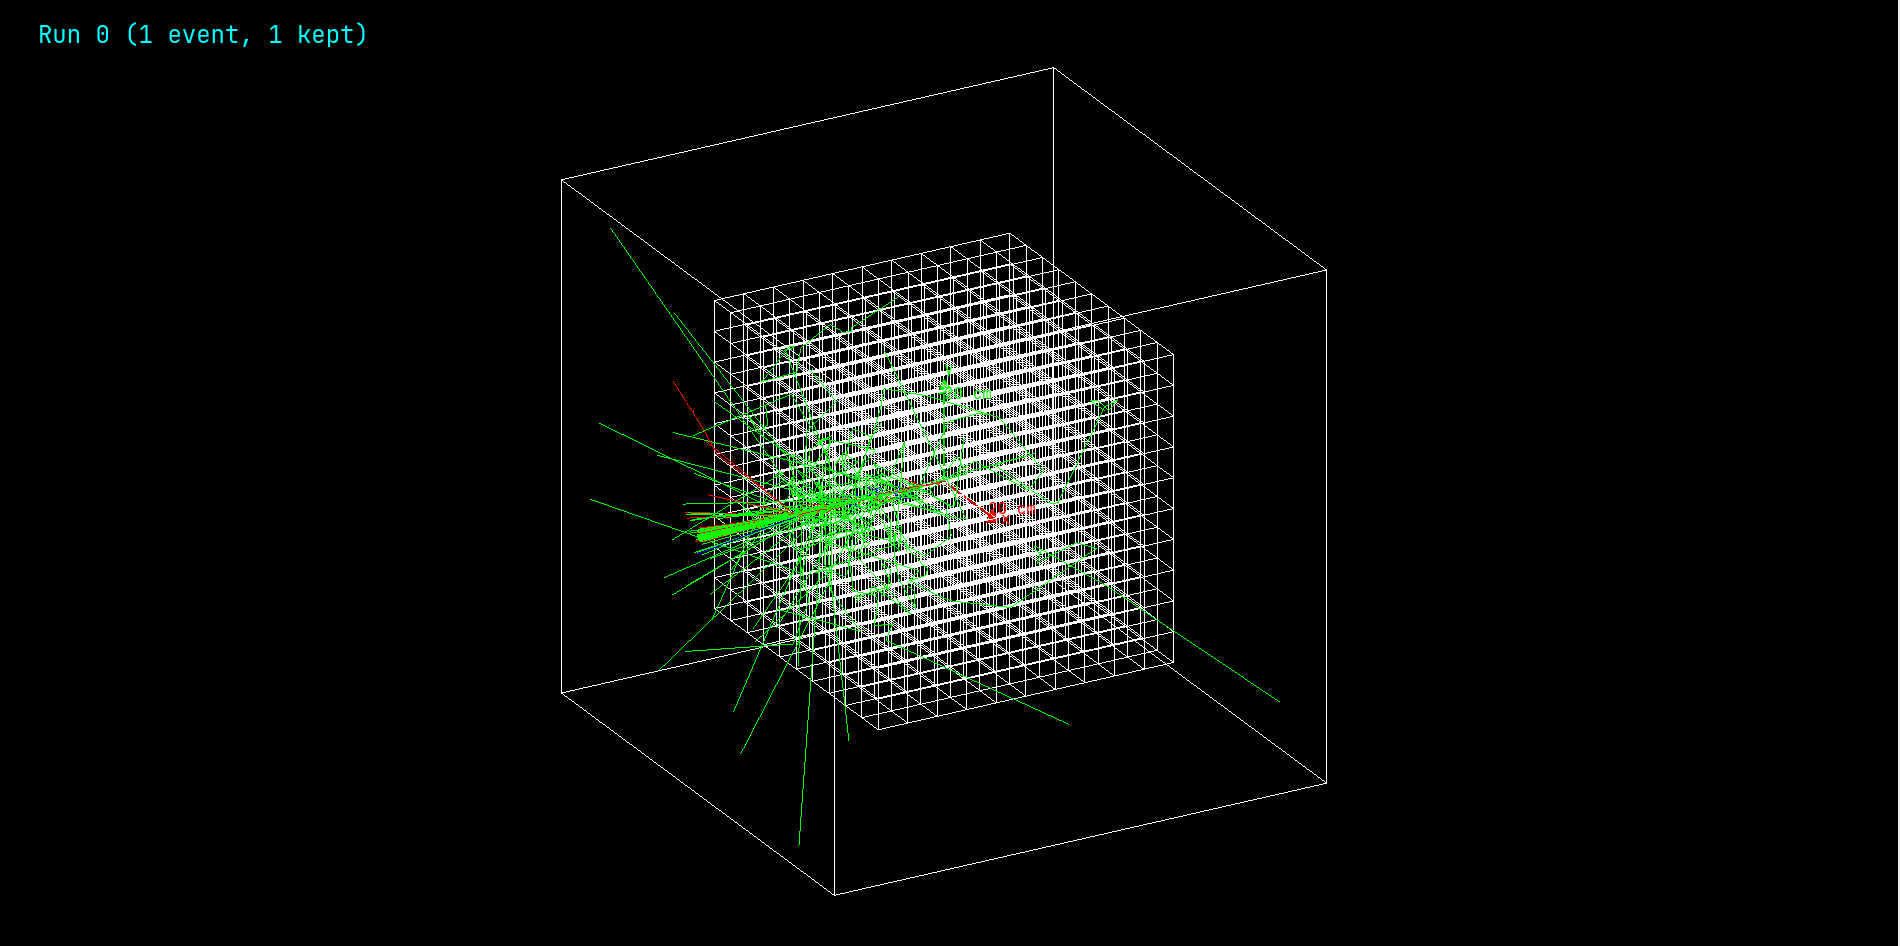
\includegraphics[scale=0.25]{imgs/sim_beam.png}
		\centering
		\caption{An event of a beam of $1$ GeV electrons interacting with the voxels of water simulated using Geant4}
	\end{figure}
	\end{center}

	\begin{center}
\begin{figure}
	\centering
	\hfill
	\subfigure{{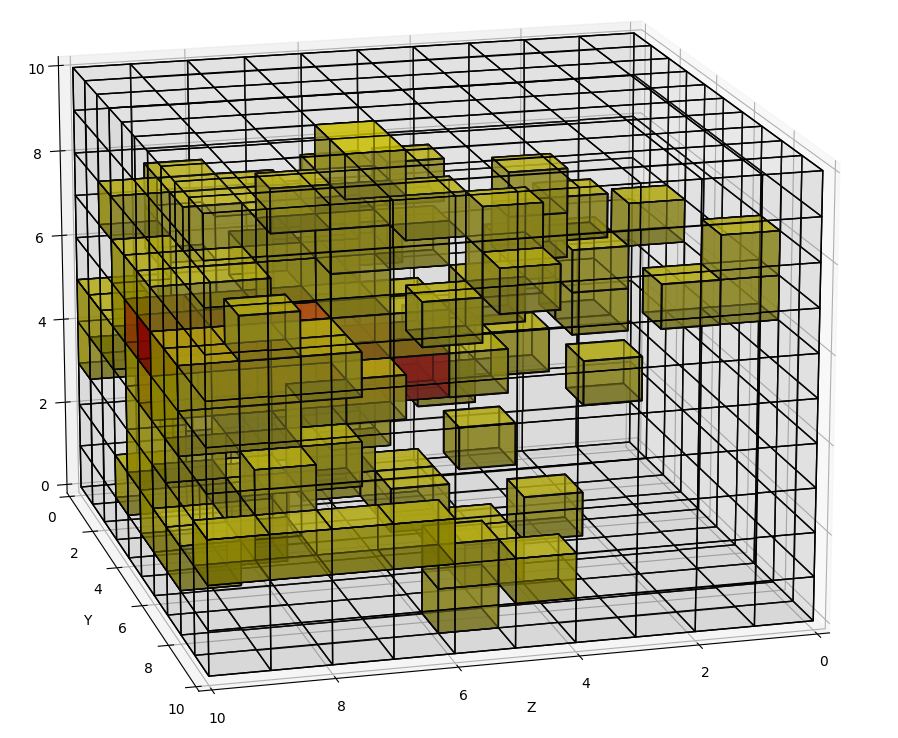
\includegraphics[scale=0.5]{imgs/voxels_edep.png}}}
\hfill
	\subfigure{{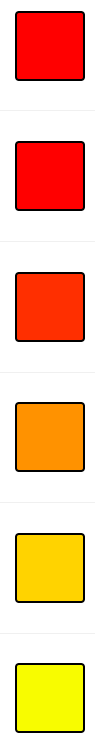
\includegraphics[scale=0.25]{imgs/palette.png}}}
	\caption{The voxels where the amount of deposited of energy is $>0$ are shown in grading colors from yellow to red}
\hfill
\end{figure}
    \end{center}

	\begin{center}
	\begin{figure}
		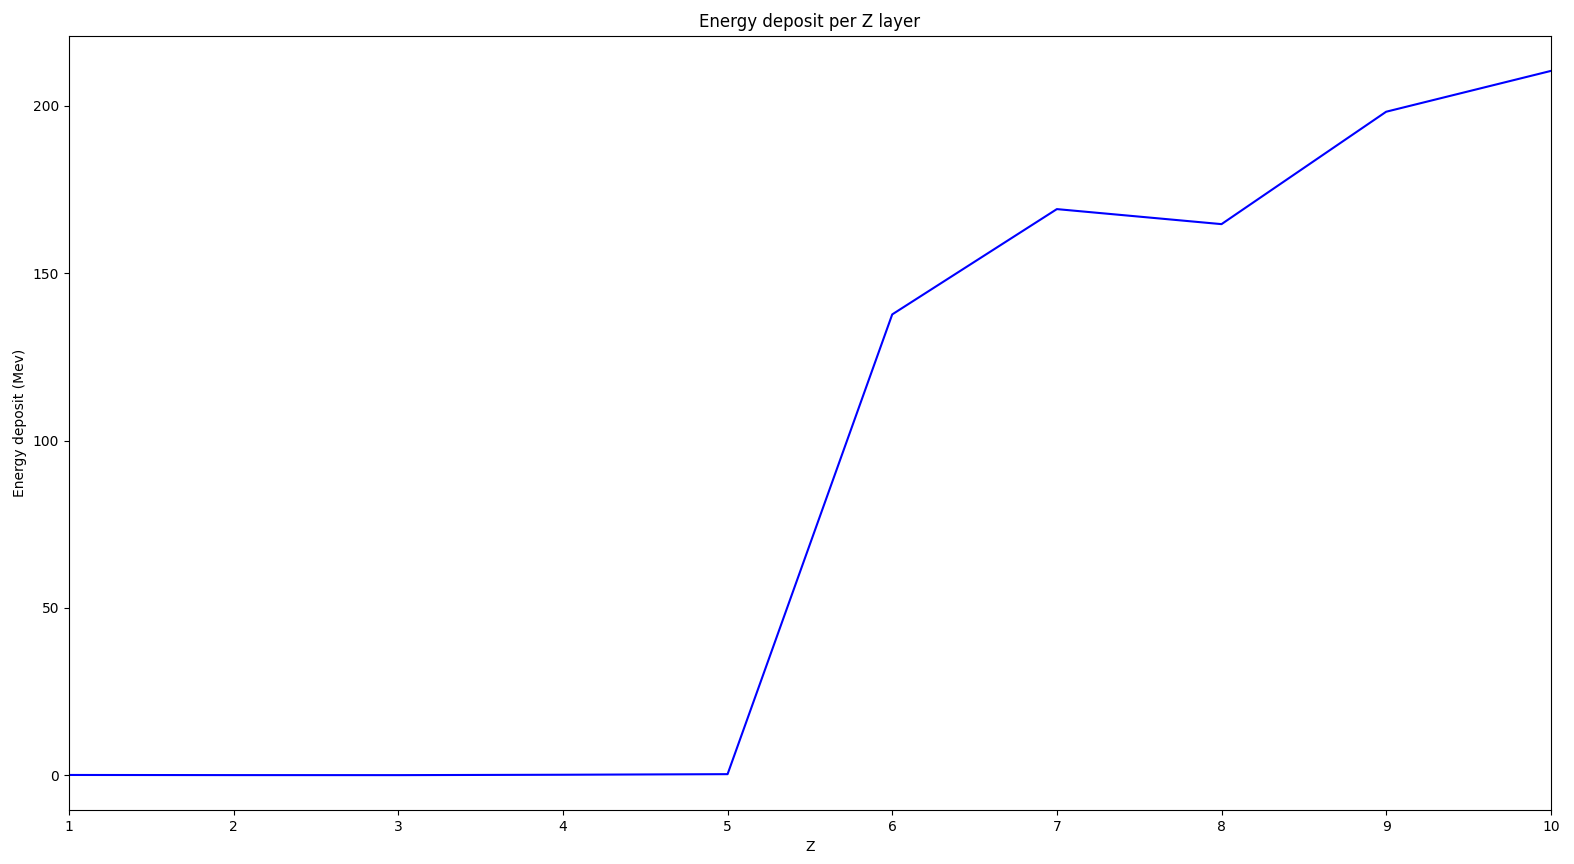
\includegraphics[scale=0.3]{imgs/edep_z_axis.png}
\centering
\caption{Sum of energy deposits on each Z layer of voxels}
	\end{figure}
\end{center}

\begin{center}
	\begin{figure}
		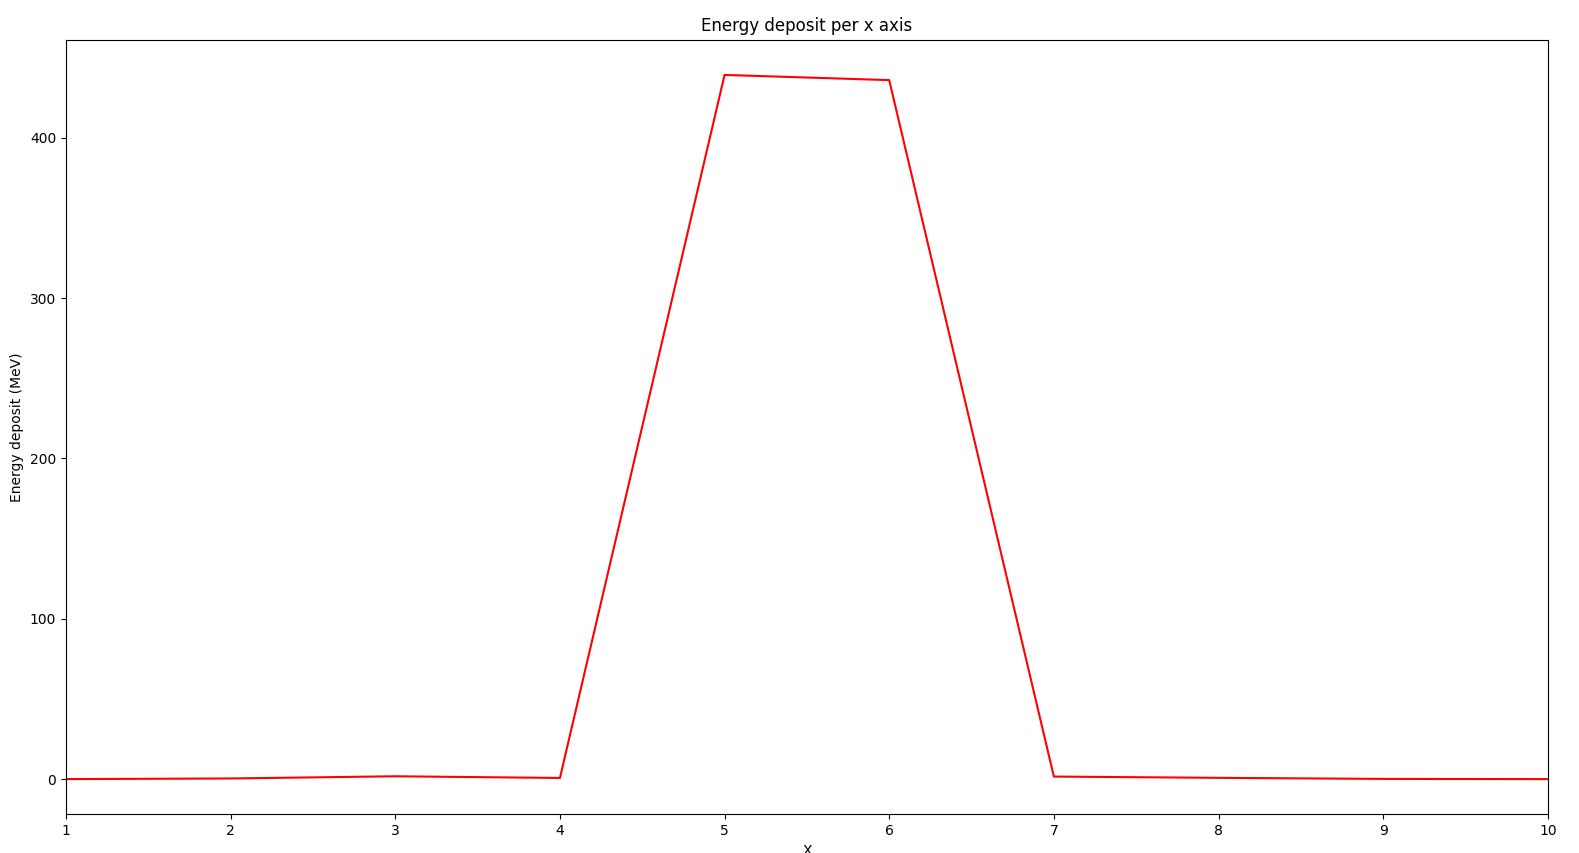
\includegraphics[scale=0.3]{imgs/edep_x_axis.png}
		\centering
		\caption{Sum of energy deposits on each X layer of voxels}
	\end{figure}
\end{center}

\begin{center}
	\begin{figure}
		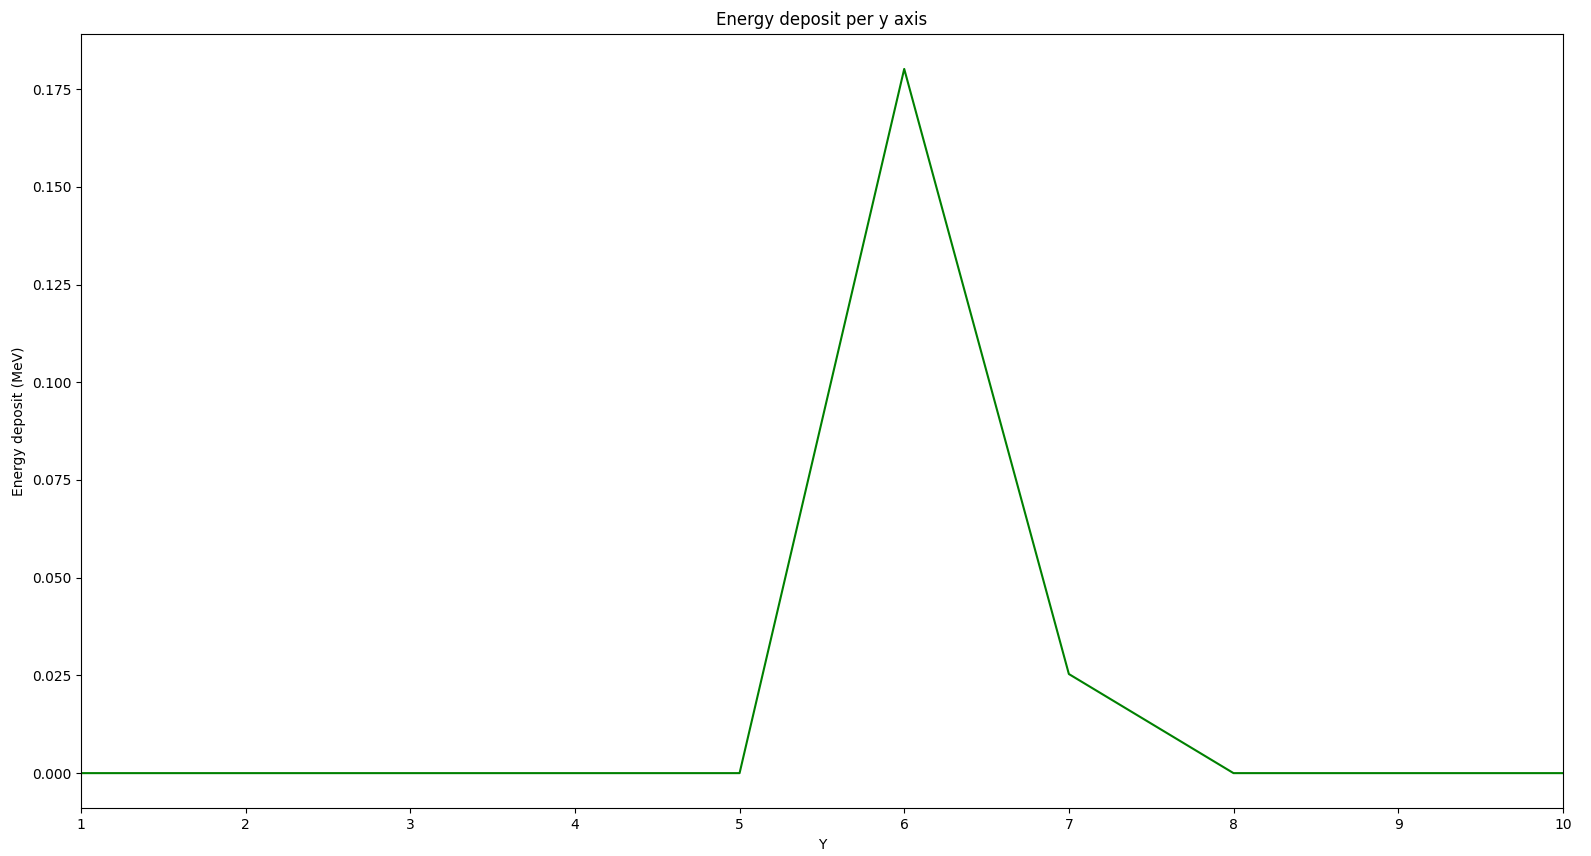
\includegraphics[scale=0.3]{imgs/edep_y_axis.png}
		\centering
		\caption{Sum of energy deposits on each Y layer of voxels}
	\end{figure}
\end{center}


	\chapter{\sc Geant4 Parametrization}
	Parametrization is the mechanism that allows the user to overtake the detailed Geant4 tracking inside a given volume for given particles species. This allows the user to provide his own implementation of the physics and detector response.

	\chapter{\sc Perspectives}
	Use machine learning models inside Geant4 simulation gives us the possibility to further study the performance and accuracy of various models for different particles in multiple ranges of energy.

	The author will continue the study of different machine learning models especially in very low energy and very high energy ranges.


	As a first perspective one could try to incorporate Physics Informed Neural Networks in the simulation, using equations of interaction of particles with matter.


\end{document}